% Practica 6 v2 · Diagrama a bloques: LED como fotodetector, TIA con LM358
% Optoelectronica V3736 · 2026B · Dr. Ruben Estrada Marmolejo
\documentclass[border=10pt]{standalone}
\usepackage[T1]{fontenc}
\usepackage[utf8]{inputenc}
\usepackage{lmodern}
\renewcommand{\familydefault}{\sfdefault}
\usepackage{tikz}
\usetikzlibrary{positioning,arrows.meta,calc}
\definecolor{optosignal}{HTML}{2A5CAA}
\definecolor{optoemit}{HTML}{C9601F}
\definecolor{optodetect}{HTML}{6B4C9A}
\definecolor{optoink}{HTML}{1C1F24}
\definecolor{optoconfirm}{HTML}{3E7C59}
\begin{document}
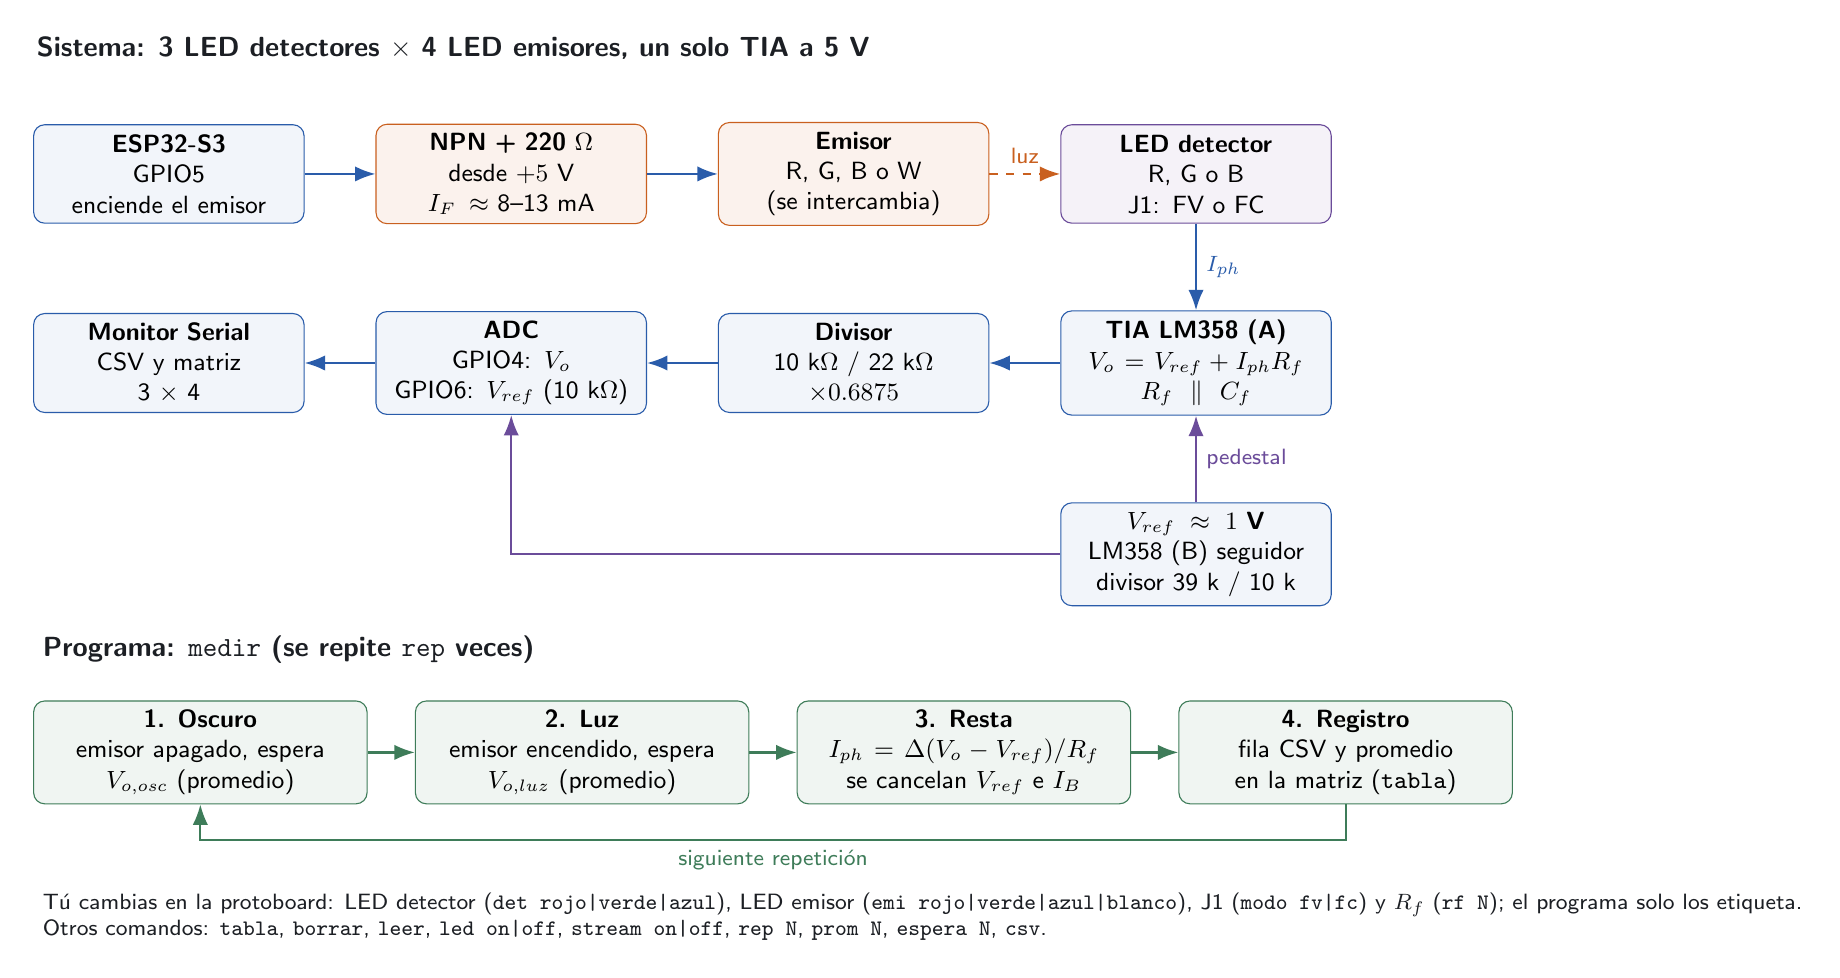
\begin{tikzpicture}[
  b/.style={draw=optosignal,rounded corners,fill=optosignal!6,align=center,minimum height=1.25cm,text width=3.2cm,font=\small},
  e/.style={b,draw=optoemit,fill=optoemit!8},
  d/.style={b,draw=optodetect,fill=optodetect!7},
  s/.style={b,draw=optoconfirm,fill=optoconfirm!8,text width=4.0cm},
  f/.style={-{Latex[length=2.6mm]},thick,optosignal},
  node distance=0.75cm and 0.9cm]
\node[font=\bfseries,text=optoink,anchor=west] at (-1.8,1.6) {Sistema: 3 LED detectores $\times$ 4 LED emisores, un solo TIA a 5 V};
\node[b] (esp) {\textbf{ESP32-S3}\\GPIO5\\enciende el emisor};
\node[e,right=of esp] (drv) {\textbf{NPN + 220 $\Omega$}\\desde $+5$ V\\$I_F\approx$ 8--13 mA};
\node[e,right=of drv] (led) {\textbf{Emisor}\\R, G, B o W\\(se intercambia)};
\node[d,right=of led] (det) {\textbf{LED detector}\\R, G o B\\J1: FV o FC};
\node[b,below=1.1cm of det] (tia) {\textbf{TIA LM358 (A)}\\$V_o=V_{ref}+I_{ph}R_f$\\$R_f\parallel C_f$};
\node[b,left=of tia] (div) {\textbf{Divisor}\\10 k$\Omega$ / 22 k$\Omega$\\$\times0.6875$};
\node[b,left=of div] (adc) {\textbf{ADC}\\GPIO4: $V_o$\\GPIO6: $V_{ref}$ (10 k$\Omega$)};
\node[b,left=of adc] (pc) {\textbf{Monitor Serial}\\CSV y matriz\\3 $\times$ 4};
\node[b,below=1.1cm of tia] (ref) {\textbf{$V_{ref}\approx1$ V}\\LM358 (B) seguidor\\divisor 39 k / 10 k};
\draw[f] (esp)--(drv); \draw[f] (drv)--(led);
\draw[f,optoemit,dashed] (led)--node[above,font=\footnotesize]{luz}(det);
\draw[f] (det)--node[right,font=\footnotesize]{$I_{ph}$}(tia);
\draw[f] (tia)--(div); \draw[f] (div)--(adc); \draw[f] (adc)--(pc);
\draw[f,optodetect] (ref)--node[right,font=\footnotesize]{pedestal}(tia);
\draw[f,optodetect] (ref.west) -| (adc.south);
\node[font=\bfseries,text=optoink,anchor=west] at ($(pc.south west)+(0,-3.0)$) (tit) {Programa: \texttt{medir} (se repite \texttt{rep} veces)};
\node[s,below=0.35cm of tit.south west,anchor=north west] (p1) {\textbf{1. Oscuro}\\emisor apagado, espera\\$V_{o,osc}$ (promedio)};
\node[s,right=0.6cm of p1] (p2) {\textbf{2. Luz}\\emisor encendido, espera\\$V_{o,luz}$ (promedio)};
\node[s,right=0.6cm of p2] (p3) {\textbf{3. Resta}\\$I_{ph}=\Delta(V_o-V_{ref})/R_f$\\se cancelan $V_{ref}$ e $I_B$};
\node[s,right=0.6cm of p3] (p4) {\textbf{4. Registro}\\fila CSV y promedio\\en la matriz (\texttt{tabla})};
\draw[f,optoconfirm] (p1)--(p2); \draw[f,optoconfirm] (p2)--(p3); \draw[f,optoconfirm] (p3)--(p4);
\draw[f,optoconfirm] (p4.south) -- ++(0,-0.45) -| node[pos=0.25,below,font=\footnotesize]{siguiente repetición} (p1.south);
\node[align=left,font=\footnotesize,text=optoink,anchor=north west] at ($(p1.south west)+(0,-1.0)$) {%
Tú cambias en la protoboard: LED detector (\texttt{det rojo|verde|azul}), LED emisor (\texttt{emi rojo|verde|azul|blanco}), J1 (\texttt{modo fv|fc}) y $R_f$ (\texttt{rf N}); el programa solo los etiqueta.\\
Otros comandos: \texttt{tabla}, \texttt{borrar}, \texttt{leer}, \texttt{led on|off}, \texttt{stream on|off}, \texttt{rep N}, \texttt{prom N}, \texttt{espera N}, \texttt{csv}.};
\end{tikzpicture}
\end{document}
